\section{HLASM context tables}

HLASM context tables (in code referred simply as hlasm context) is composition of tables and stacks that describe state of the currently processed open-code. The object is persistent between source files within an open-code. It is created in analyzer and has the same lifespan. The architecture can be seen in \cref{fig06:hlasm}.

\begin{figure}
	\centering
	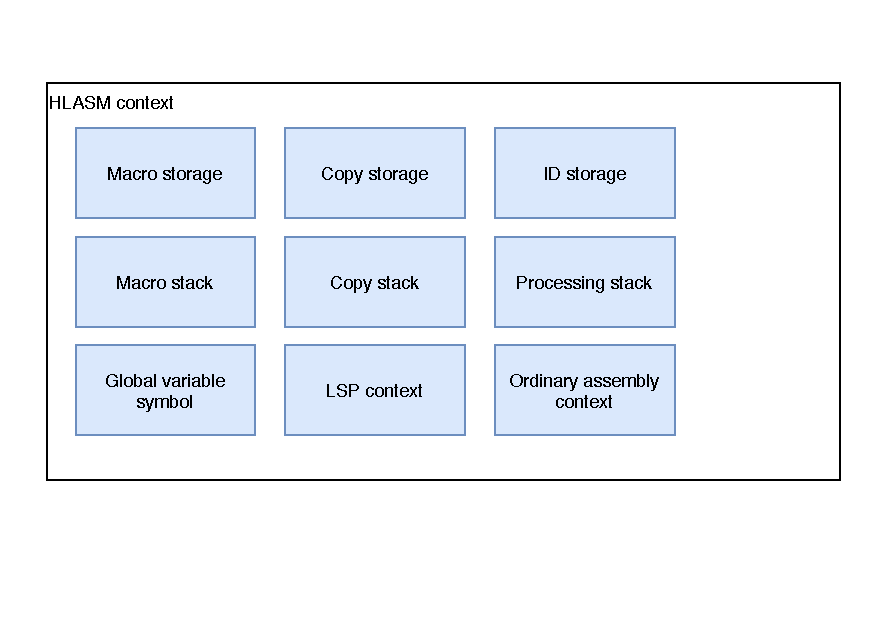
\includegraphics[width=\textwidth / 2]{img/hlasm_arch}
	\caption{The composition of HLASM context tables component}
	\label{fig06:hlasm}
\end{figure}